\documentclass[main.tex]{subfiles}

\begin{document}

\subsection{Memory Model}

\gama uses an unified programming model that assumes a hierarchy composed of multiple devices (both \cpus and \gpus), where each device has access to a private address space (shared by all computational units, or cores, within that device), and a distributed memory system between devices. The framework assumes that multiple computational units of an individual device can cooperate and communicate through a shared memory space, and that the underlying programming and execution model of that device provides synchronization mechanisms (barriers, atomics and memory fences).
To abstract the distributed memory model that is used between devices, \gama introduces a global address space. \Cref{fig:gama_memory_model} illustrates how \gama understands the memory hierarchy of a \hetplat.


\subsubsection{Memory Consistency}

Communication between the different memory spaces of each device is expensive due to the need of synchronization and communication between the host \cpu and the devices. Due to this, a relaxed consistency model is used, which enables the system to optimize data movements between devices, offering the developer a single synchronization primitive to enforce memory consistency.

\subsubsection{Software Cache}

Some applications require safe exclusive access to specific partitions of a data set. To address this issue, a software cache among devices was implemented. This ensures that the required data is as close to the device as possible, taking advantage of the local memory of each device. It also provides a safeguard mechanism in combination with the global memory system, to ensure each device has a copy of a specific partition, when requested by the developer. Additionally, the cache local copies on the device shared memory space use semantically correct synchronization primitives within the device.

\begin{figure}[!htp]
  \centering
  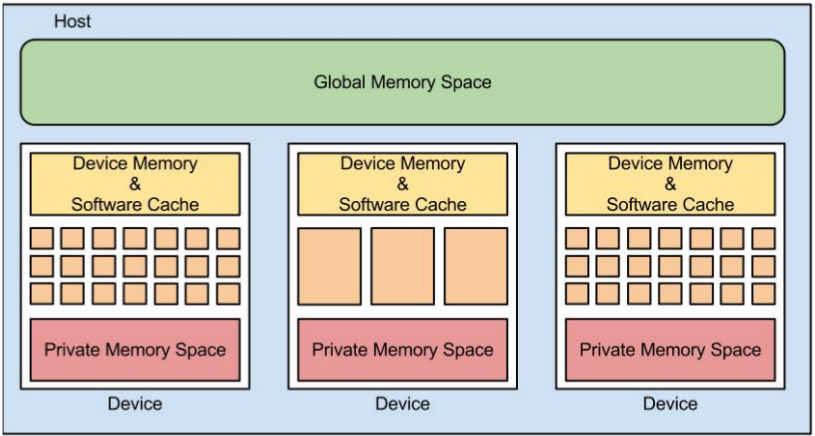
\includegraphics[width=0.5\textwidth]{gama_model}
  \caption{\gama Memory Model \label{fig:gama_memory_model}}
\end{figure}

\end{document}
